%!TEX program = pdflatex
\documentclass[12pt]{article}
\usepackage{geometry}
% \geometry{left=2.0cm,right=2.0cm,top=2.5cm,bottom=2.5cm}


\usepackage{times}
\usepackage{soul}
\usepackage{url}
\usepackage[hidelinks]{hyperref}
\usepackage[utf8]{inputenc}
\usepackage[small]{caption}
\usepackage{graphicx}
\usepackage{subfigure}
\usepackage{amsmath}
\usepackage{amsthm}
\usepackage{booktabs}
\usepackage{algorithm}
\usepackage{algorithmic}
\usepackage{lipsum}
\usepackage{multirow}  % for multirow command used in the table
\usepackage{setspace}
\usepackage{ulem}  % 用于添加下划线
\usepackage{enumitem}
\usepackage{color}
\usepackage{amssymb}  % 用于打对号
\newcommand{\eg}{e.g.}
\newcommand{\ie}{i.e.}
\urlstyle{same}

\newtheorem{example}{Example}
\newtheorem{theorem}{Theorem}


\begin{document}
\setstretch{1.5}
\linespread{1}
\title{Response to Reviewers of TCSVT-07024-2021: A Simple and Strong Baseline for Universal Targeted Attacks on Siamese Visual Tracking}
\author{Zhenbang Li, Yaya Shi, Jin Gao, Shaoru Wang, \\Bing Li, Pengpeng Liang, Weiming Hu}
\date{}
\maketitle

\noindent Dear Editors:

We would like to express our heartfelt gratitude to you and the reviewers for the insightful and helpful comments. When we revised the paper, we carefully considered and followed all the comments and suggestions provided by you and the reviewers. To summarize, we have made the following revisions:

(1) We have added the advantages \& limitations of the proposed method after experimental analysis and the future work to the conclusion.

(2) We have carefully considered and followed all the comments and suggestions related to the clarity of the writing, and made the new material a thoroughly revised manuscript.

% 消融实验
(3) We have added a new experiment to attack in the YCbCr color space to reduce the perceptibility of the perturbations.

% 消融实验:噪声攻击。
(4) We have added a new experiment to evaluate the attack performance of the random patterns.

% 消融实验
(5) We have added a new experiment to evaluate the attack performance when only adding the perturbation to the search/template image.

% 引用论文
(6) We have added 3 papers published in the IEEE Transactions on Circuits and Systems for Video Technology, which are most closely related to our manuscript, and analysed what is distinctive / new about our current manuscript related to these previously published papers. For your convenience in cross-checking, the new text is given as follows.

\uline{
Some recent research topics which are mostly related to adversarial attack also include digital watermarking [33], 3D face presentation attacks to the face recognition networks [34] and adversarial defense for image classifiers [26].
Xiong \textit{et al.} [33] propose to generate the digital watermarking by slightly modifying the pixel values of video frames to protect video content from unauthorized access. Compared with [33], our purpose of modifying pixel values of video frames is attacking the tracker, instead of detecting the illegal distribution of a digital movie.
Jia \textit{et al.} [34] propose to generate 3D face artifacts to attack the face recognition network. Compared with [34], our method directly modifies the input of the network instead of changing the input of cameras using 3D face artifacts.
Wang \textit{et al.} [26] propose the white-box attack/defense methods for image classifiers. Compared with [26], we focus on attacking the object tracking networks instead of the image classification networks.
}

We hope that our revised manuscript is now appropriate for publication in IEEE Transactions on Circuits and Systems for Video Technology. Specific responses to all the comments of each reviewer are included in the rest of this document and highlighted using bold font after the comments of each reviewer for the convenience of cross-reference. To make the changes easier to identify where necessary, we also have underlined most of the revised parts in the manuscript and provide an underlined version for the convenience of second review.\\[10pt]
\indent We are looking forward to your reply.\\[10pt]
\noindent Yours sincerely,\\
\noindent Zhenbang Li, Yaya Shi, Jin Gao, Shaoru Wang, Bing Li, Pengpeng Liang, Weiming Hu
\\
\\
\\
\noindent Dr. Jin Gao (Contact author)\\
\noindent National Laboratory of Pattern Recognition (NLPR)\\
\noindent Institute of Automation, Chinese Academy of Sciences (CASIA)\\
\noindent Address: No. 95, Zhongguancun East Road, Haidian District,\\
\noindent Beijing 100190, P. R. China\\
\noindent Email: jin.gao@nlpr.ia.ac.cn

%%%%%%%%%%%%%%%%% 审稿人 1 %%%%%%%%%%%%%%%%%
\newpage
{\centering\section*{Response Letter to Reviewer \#1}}
\noindent Dear Reviewer \#1:

Thank you very much for your thorough review. Your insightful comments are very helpful for us to improve the quality of the paper. According to your comments and suggestions, we have carefully and extensively revised the manuscript. The main revised parts are highlighted by underlines in the underlined version for your convenience. You will find that all your comments and suggestions are considered and followed. We hope that our revised manuscript is now appropriate for publication in IEEE Transactions on Circuits and Systems for Video Technology.
In addition, point-to-point responses to your comments are given below and highlighted using bold font in line with your comments in order to facilitate cross-referencing.\\[10pt]
\indent We are looking forward to your reply.\\[10pt]
\noindent Yours sincerely,\\
\noindent Zhenbang Li, Yaya Shi, Jin Gao, Shaoru Wang, Bing Li, Pengpeng Liang, Weiming Hu
\\
\\
\\
\noindent Dr. Jin Gao (Contact author)\\
\noindent National Laboratory of Pattern Recognition (NLPR)\\
\noindent Institute of Automation, Chinese Academy of Sciences (CASIA)\\
\noindent Address: No. 95, Zhongguancun East Road, Haidian District,\\
\noindent Beijing 100190, P. R. China\\
\noindent Email: jin.gao@nlpr.ia.ac.cn

\newpage
\textit{This paper addresses the task of attacking Siamese network-based trackers in a simple yet effective fashion. Unlike other methods that operate in the video-specific attacking regime (which resides on network inference for generating perturbations while tracking), this method is the first to perform universal targeted attacks for Siamese trackers utilizing both the translucent perturbation and the adversarial patch together. By adding the perturbation to the template and adding the patch to the search image while performing tracking, this work fools the Siamese trackers to the fake target region and thus makes them fail in tracking the real target object. Overall, this is an interesting paper, and it is well written and organized. As it is a resubmitted manuscript, I notice that the authors have made substantial changes to the previous manuscript, which are able to appropriately respond to the comments made by the previous reviewers. Although the template perturbation and adversarial patch are both easy to observe for human eyes as the previous reviewers have pointed out, and the SSIMs for them are also lower than the video-specific attacking method, e.g., FAN [6], this reviewer believes that this proposed new framework can be a new configuration of adversarial attack on visual tracking for its achieved balance between the attack efficiency and the perturbation perceptibility. This new configuration will attract increasing attention from the visual tracking attack community to study on more efficient attack methods.}

\textbf{Many thanks for your positive comments on the strength of our paper and the novelty of the proposed attack method.}

%%%% 问题 1.1 %%%%
\textit{In addition, I suggest the authors add more experiments to demonstrate the practicability of the attack method when the ground truth box information is missing in the training data. The experimental results show that it is effective to use the predicted boxes instead of ground truth boxes for training perturbations.}

\textbf{Thanks for the good comment. As suggessted, we have added more experiments to demonstrate the practicability of the attack method when the ground truth box information is missing in the training data. Specifically, we evaluate the untargeted and targeted attack performance using the following metrics on specific datasets: (1) AO and Precision on OTB2015, (2) SR and AO on GOT-Val, and (3) Precision, Normalized Precision and AO on LaSOT. The detailed analysis of new added experiments is added in Section IV.E of the revised manuscript. For your convenience in cross-checking, the new text is given as follows.}

\begin{table}[t]
  \renewcommand\thetable{X}
  \centering
  \caption{Attack results on OTB2015, GOT-Val and LaSOT with or without the groundtruth information.% w/ GT represents that we train perturbations using the groud truth bounding box information of the trainig dataset. w/o GT represents that we train perturbations using the predicted boxes instead of ground truth boxes of the training dataset.
  }
  \begin{tabular}{rrcccc}
  \toprule
  \multirow{2}{*}[-2pt]{Benchmarks} & \multirow{2}{*}[-2pt]{Metrics} & \multicolumn{2}{c}{Unargeted Attack} & \multicolumn{2}{c}{Targeted Attack} \\ \cmidrule{3-6}
                              &                          & w/ GT  & \multicolumn{1}{l}{w/o GT}  & w/ GT  & \multicolumn{1}{l}{w/o GT} \\ \midrule
  \multirow{2}{*}{OTB2015}     & AO                       & 0.063  & 0.056                       & 0.759  & 0.752                      \\
                              & Precision                & 0.092  & 0.080                       & 0.795  & 0.794                      \\ \midrule
  \multirow{2}{*}{GOT-Val}    & SR                       & 0.123  & 0.121                       & 0.890  & 0.893                      \\
                              & AO                       & 0.153  & 0.160                       & 0.840  & 0.833                      \\ \midrule
  \multirow{3}{*}{LaSOT}      & Precision                & 0.046  & 0.043                       & 0.605  & 0.531                      \\
                              & Norm. Prec.              & 0.048  & 0.044                       & 0.702  & 0.660                      \\
                              & AO                       & 0.069  & 0.063                       & 0.691  & 0.646                      \\ \bottomrule
  \end{tabular}
  \label{tab:agent_GT}
\end{table}

\uline{We evaluate the untargeted and targeted attack performance using the following metrics on specific datasets: (1) AO and Precision on OTB2015, (2) SR and AO on GOT-Val, and (3) Precision, Normalized Precision and AO on LaSOT. As shown in Table \ref{tab:agent_GT}, it is effective to use the predicted boxes instead of groundtruth boxes for training our perturbations, though the targeted attack performance is affected due to some ambiguous prediction results used for training.}

%%%% 问题 1.2 %%%%
\textit{A small question is that it will be better if the authors can provide some pseudo code for the untargeted attack and targeted attack processes in addition to the training process. This will facilitate the understanding of the attacking process while performing tracking.}

\begin{algorithm}[t]
    \renewcommand\thealgorithm{2}
    \caption{Attack Process}
    \label{alg:algorithm_attack}
    \textbf{Input}: The trained perturbations $\delta$ and $p$, Siamese tracker $f$, video $V=\{I_i\}_1^T$. $b^{gt}_1$ is the position of the real target in the first frame. $B^{fake}=\{b^{fake}_i\}_1^{T}$ is the trajectory we hope the tracker to output.\\
    \textbf{Output}: $B^{pred}=\{b^{pred}_i\}_1^{T}$
    \begin{algorithmic}[1] %[1] enables line numbers
      \STATE Generate the clean template image $\textbf{z}_1$ according to $I_1$ and $b^{gt}_1$.
      \STATE Generate the perturbed template image $\tilde{\textbf z}_1=\textbf z_1+\delta$.
      \STATE Let $i = 2$.
    \WHILE{$i \le T$}
    \STATE Generate clean search image $\textbf{x}_i$ according to $I_i$ and $b^{pred}_{i-1}$.
    \STATE $b^{fake}_i=\{x_{0_i}, y_{0_i}, x_{1_i}, y_{1_i}\}$
    \STATE Generate the perturbed search image $\tilde{\textbf x}_i = A_{\text{add}}(\textbf x_i, p, \{x_{0_i}, y_{0_i}, x_{1_i}, y_{1_i}\}).$
    \STATE $\textbf{C, R, Q} = f(\tilde {\textbf x}_i, \tilde{\textbf z}_1).$
    \STATE Generate the predicted bounding box $b^{pred}_i$ according to $\textbf{C, R, Q}$.
    \STATE $i = i + 1.$
    \ENDWHILE
    \STATE \textbf{return} $B^{pred}$
    \end{algorithmic}
\end{algorithm}

\textbf{
Thanks for the good comment. As suggested, we have provided the algorithm for the attack process in Section III.C of the revised manuscript.
Both the targeted attack and untargeted attack process follow the same steps as shown in Alg. \ref{alg:algorithm_attack}.
%The difference between the target attack and the untargeted attack is the evaluation. For the targeted attack, we compare the AO between $B^{pred}=\{b^{pred}_i\}_1^{T}$ and $B^{fake}=\{b^{fake}_i\}_1^{T}$. For the untargeted attack, we compare the AO between $B^{pred}=\{b^{pred}_i\}_1^{T}$ and $B^{gt}=\{b^{gt}_i\}_1^{T}$.
}

%%%% 问题 1.3 %%%%
\textit{In addition, the font size in Fig. 9 is too small to read on my computer, which needs to be improved.}

% \textbf{Thanks for the good comment. As suggested, we have increased the font size of texts in Fig. \ref{fig:attr} to make it easier to read on the computer.}


% \newgeometry{left=1cm,right=1cm,top=3cm,bottom=3cm}

% \begin{figure*}[t]
%   \renewcommand\thefigure{9}
%   \begin{center}
%     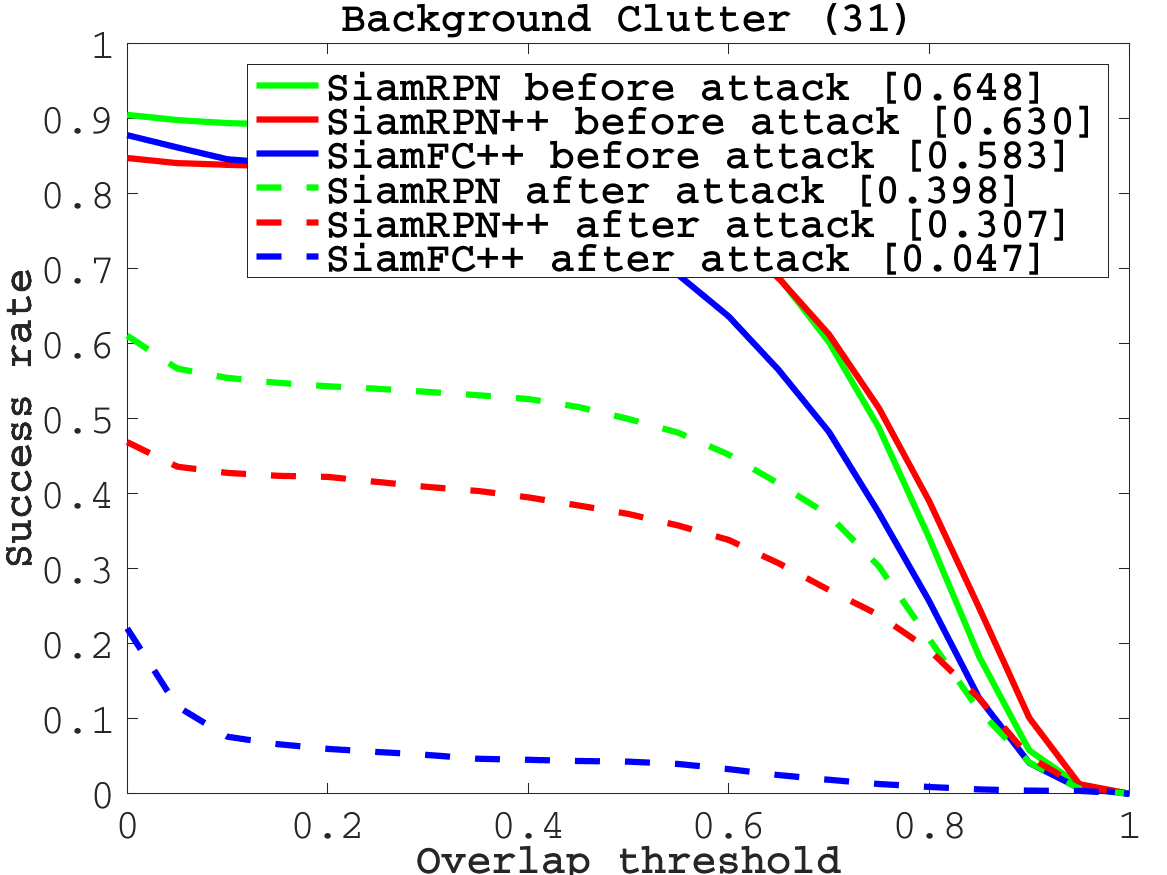
\includegraphics[width=0.32\textwidth]{images_imperceptible/OTB2015/success_plot_OPE_OTB100_BC.png}
%     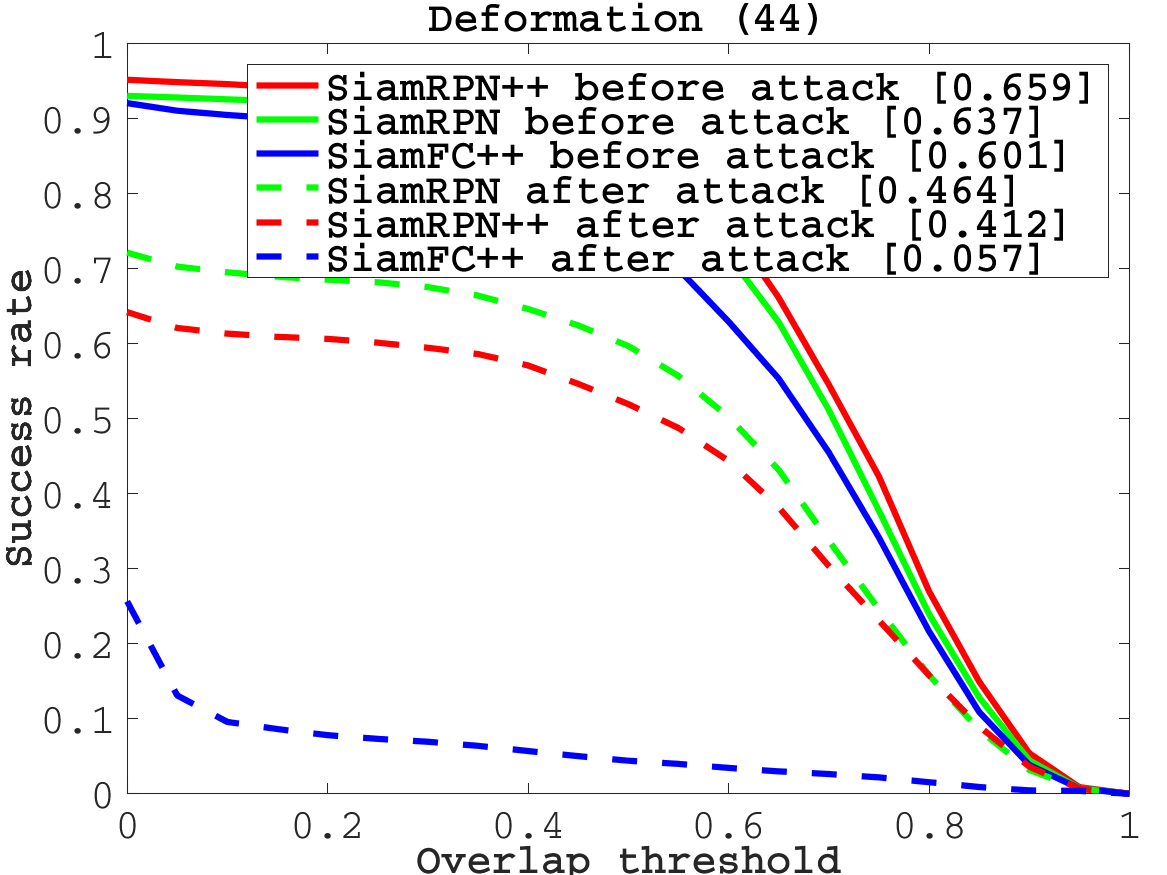
\includegraphics[width=0.32\textwidth]{images_imperceptible/OTB2015/success_plot_OPE_OTB100_DEF.png}
%     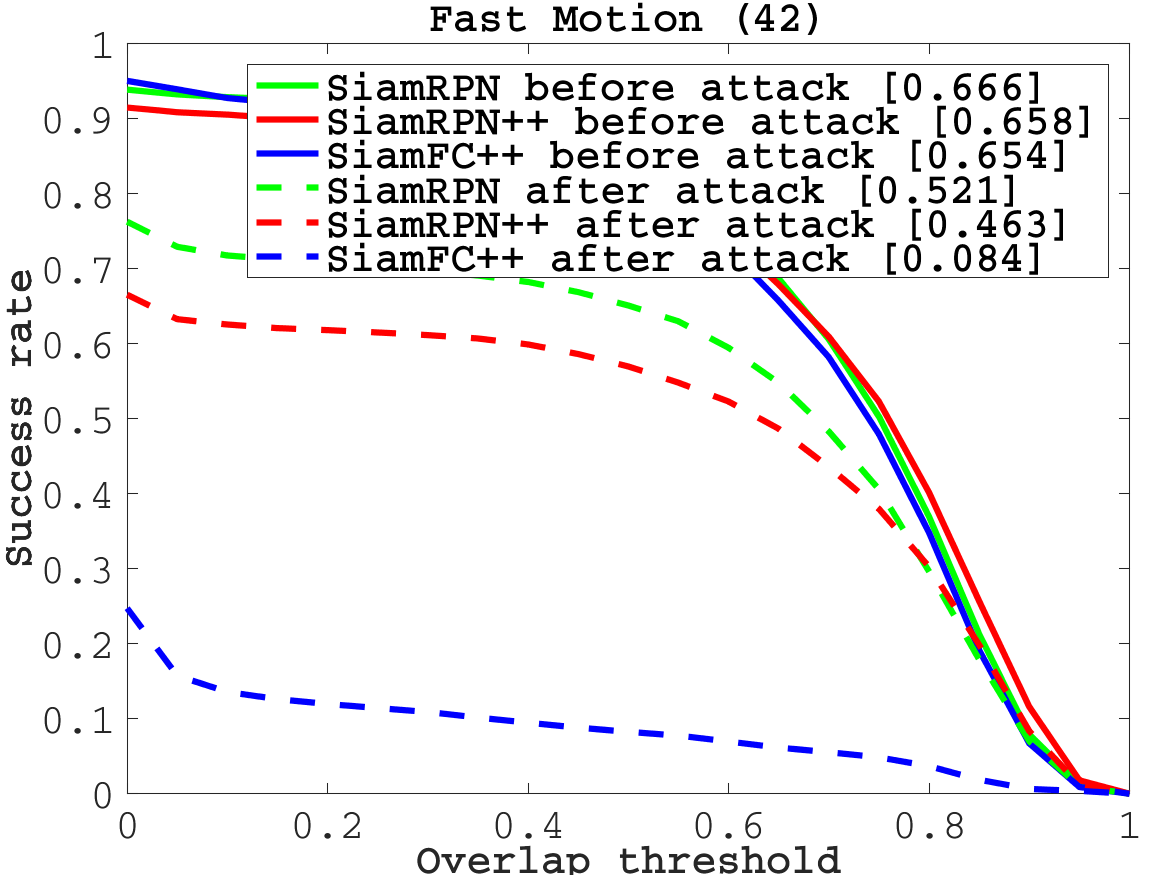
\includegraphics[width=0.32\textwidth]{images_imperceptible/OTB2015/success_plot_OPE_OTB100_FM.png}
%     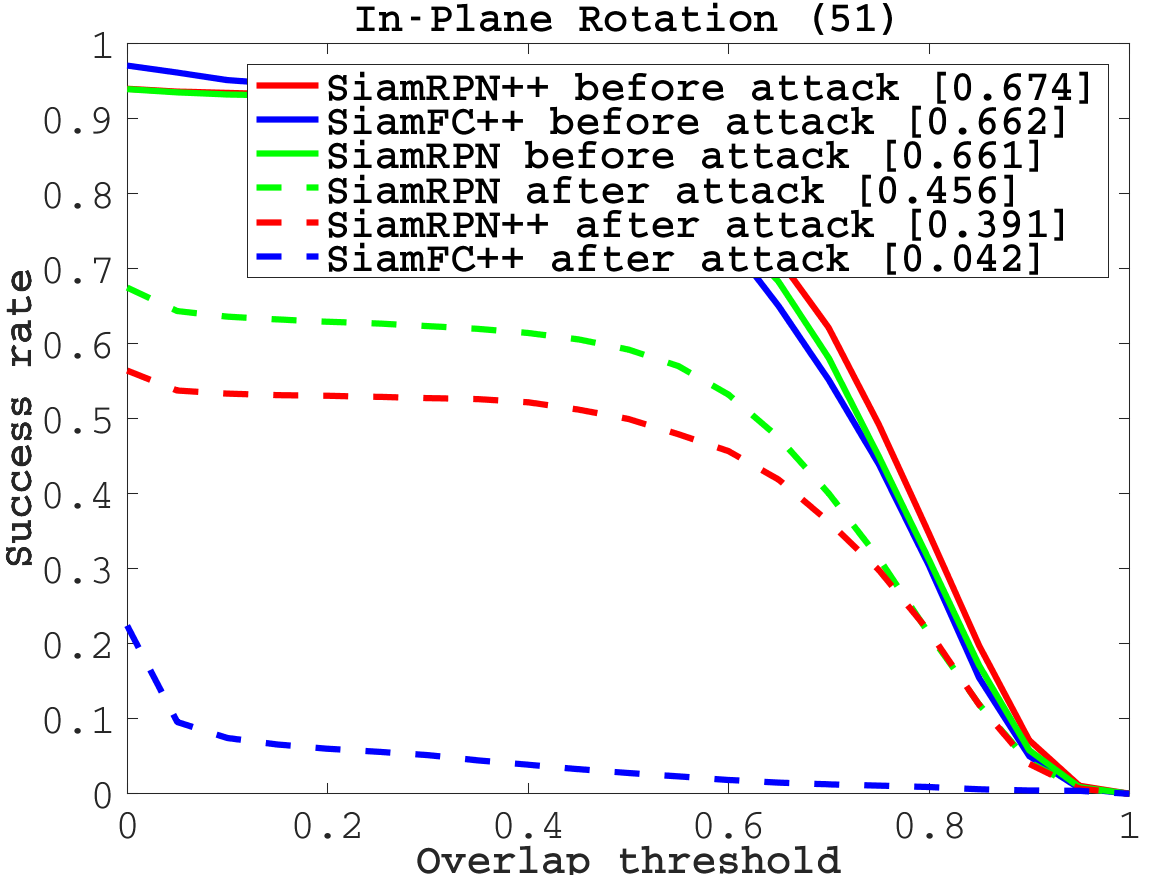
\includegraphics[width=0.32\textwidth]{images_imperceptible/OTB2015/success_plot_OPE_OTB100_IPR.png}
%     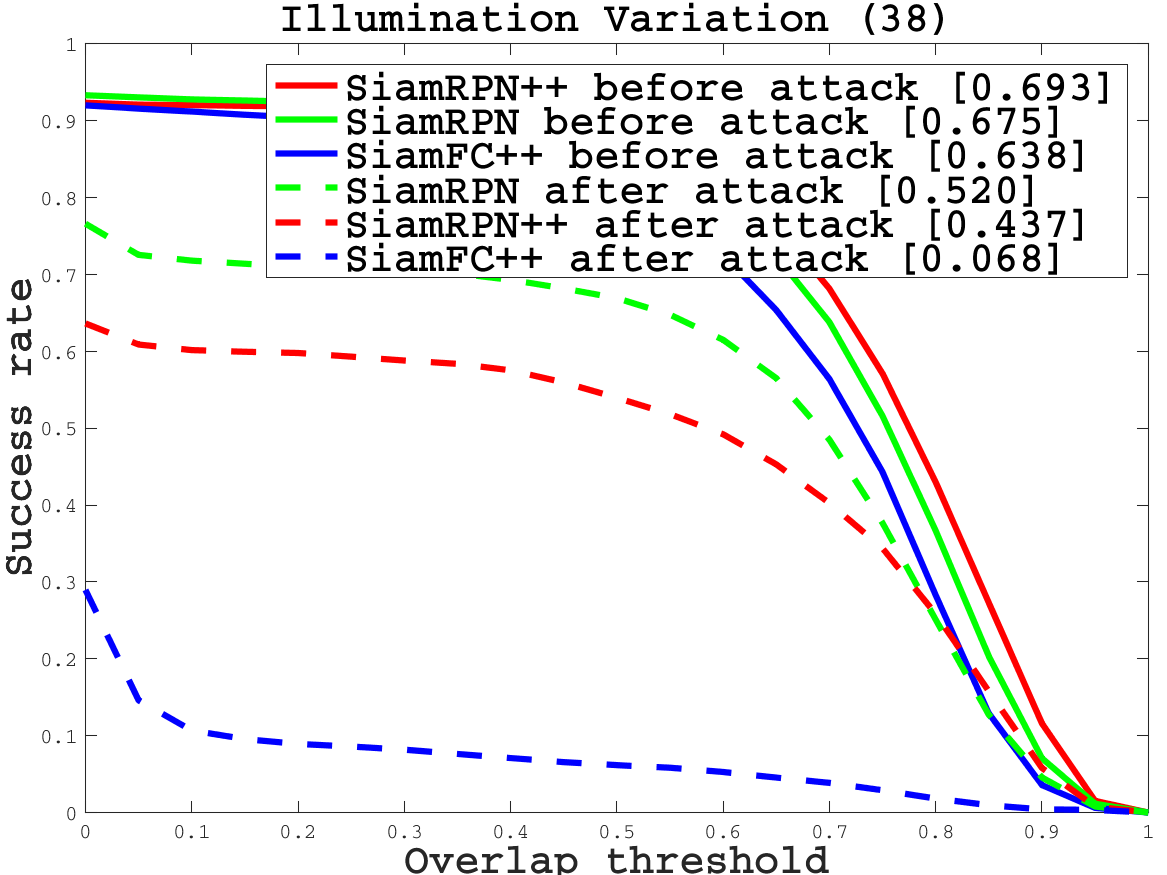
\includegraphics[width=0.32\textwidth]{images_imperceptible/OTB2015/success_plot_OPE_OTB100_IV.png}
%     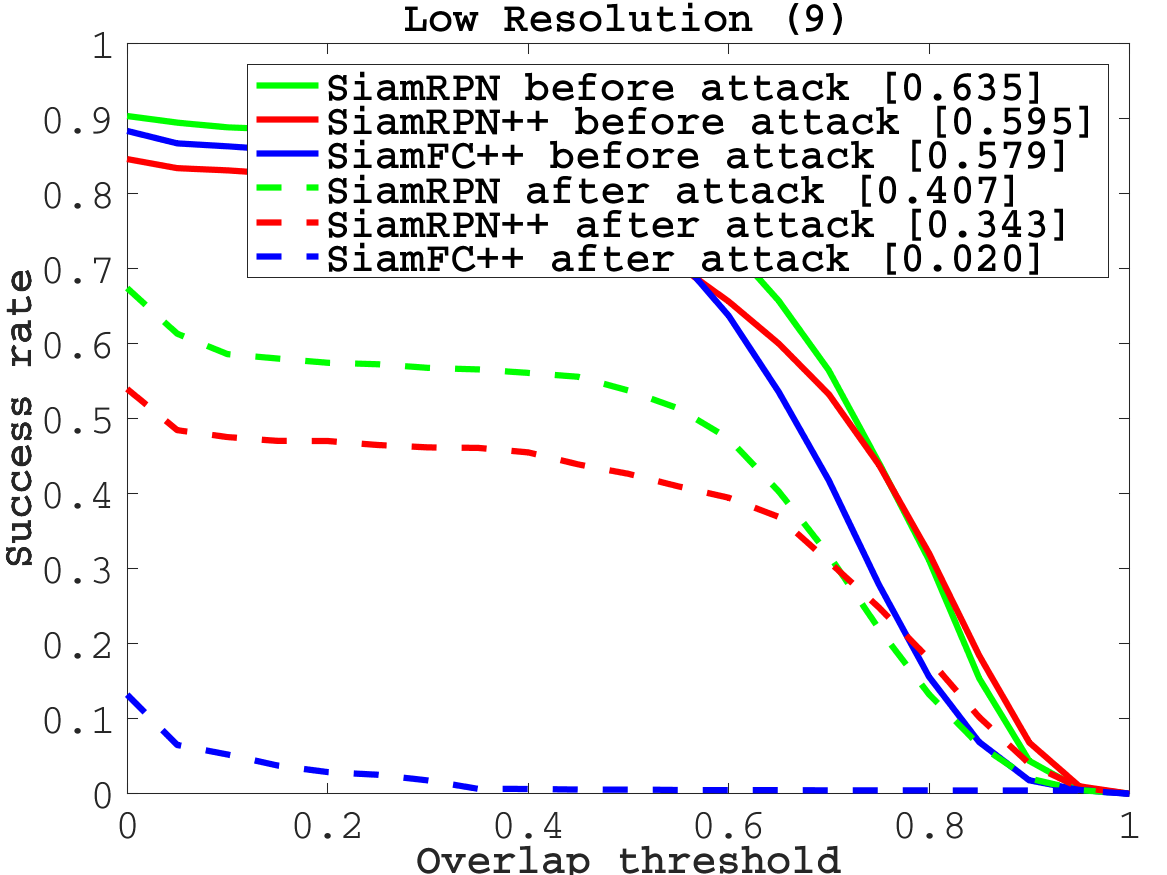
\includegraphics[width=0.32\textwidth]{images_imperceptible/OTB2015/success_plot_OPE_OTB100_LR.png}
%     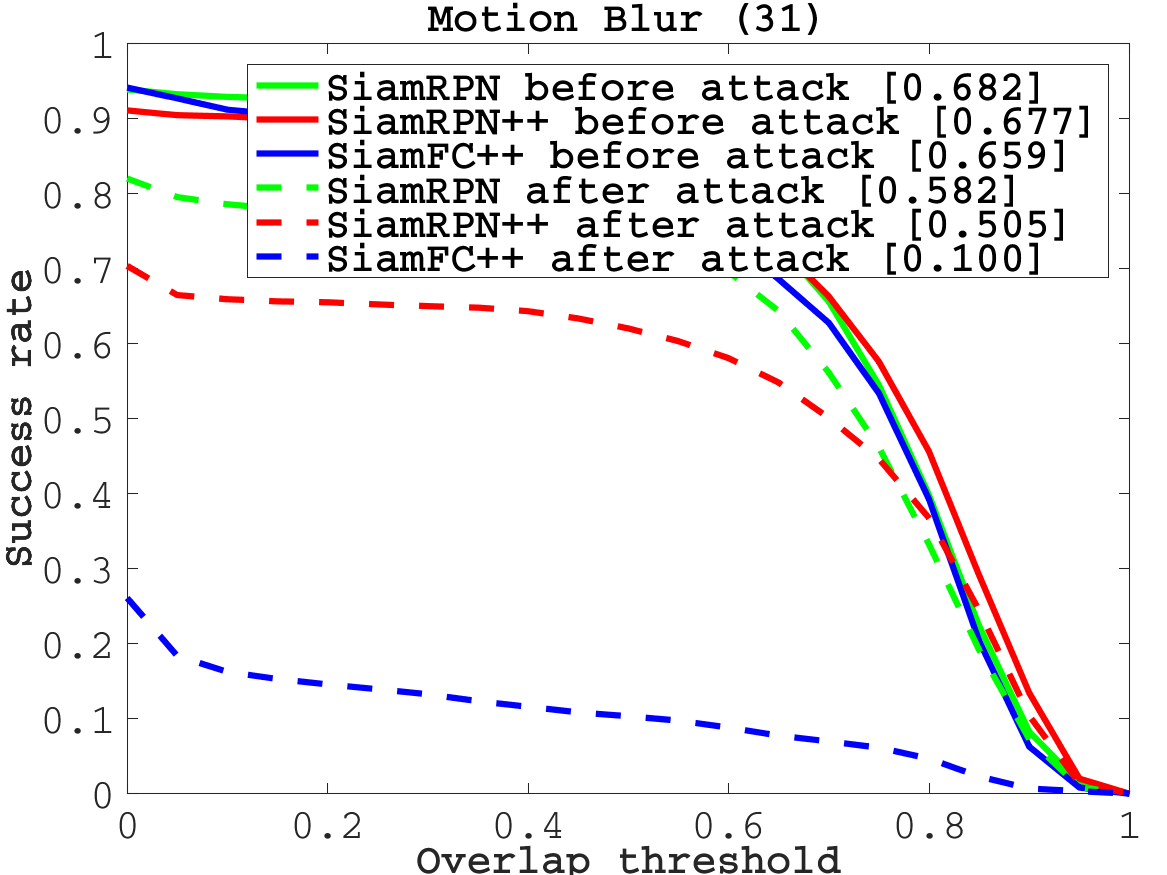
\includegraphics[width=0.32\textwidth]{images_imperceptible/OTB2015/success_plot_OPE_OTB100_MB.png}
%     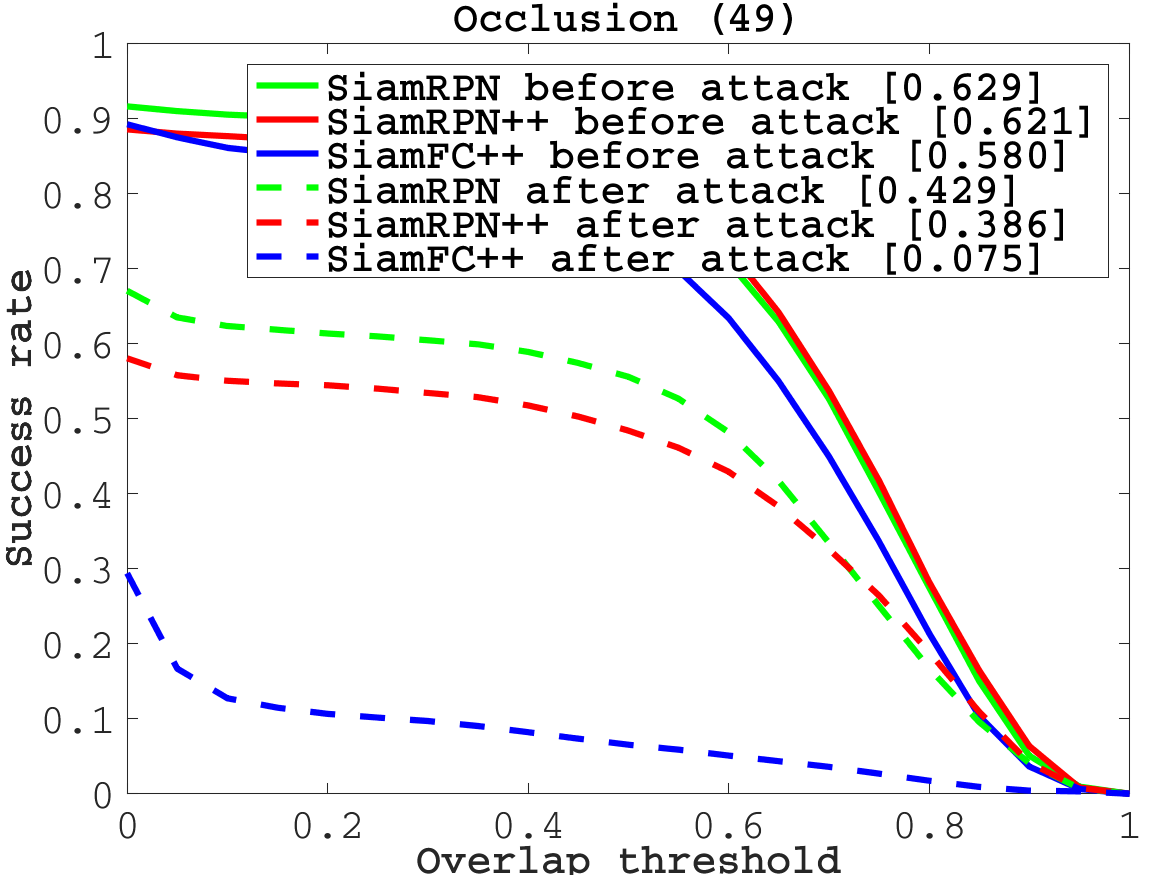
\includegraphics[width=0.32\textwidth]{images_imperceptible/OTB2015/success_plot_OPE_OTB100_OCC.png}
%     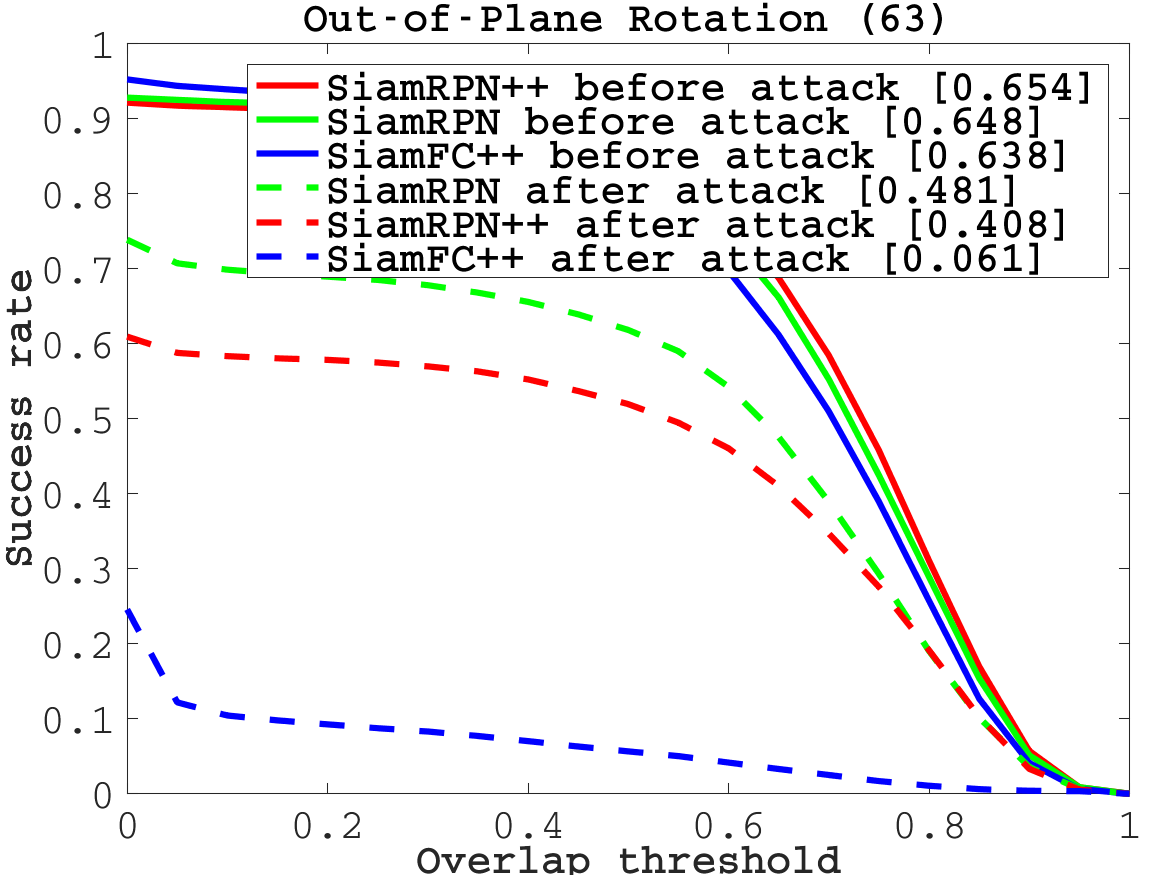
\includegraphics[width=0.32\textwidth]{images_imperceptible/OTB2015/success_plot_OPE_OTB100_OPR.png}
%     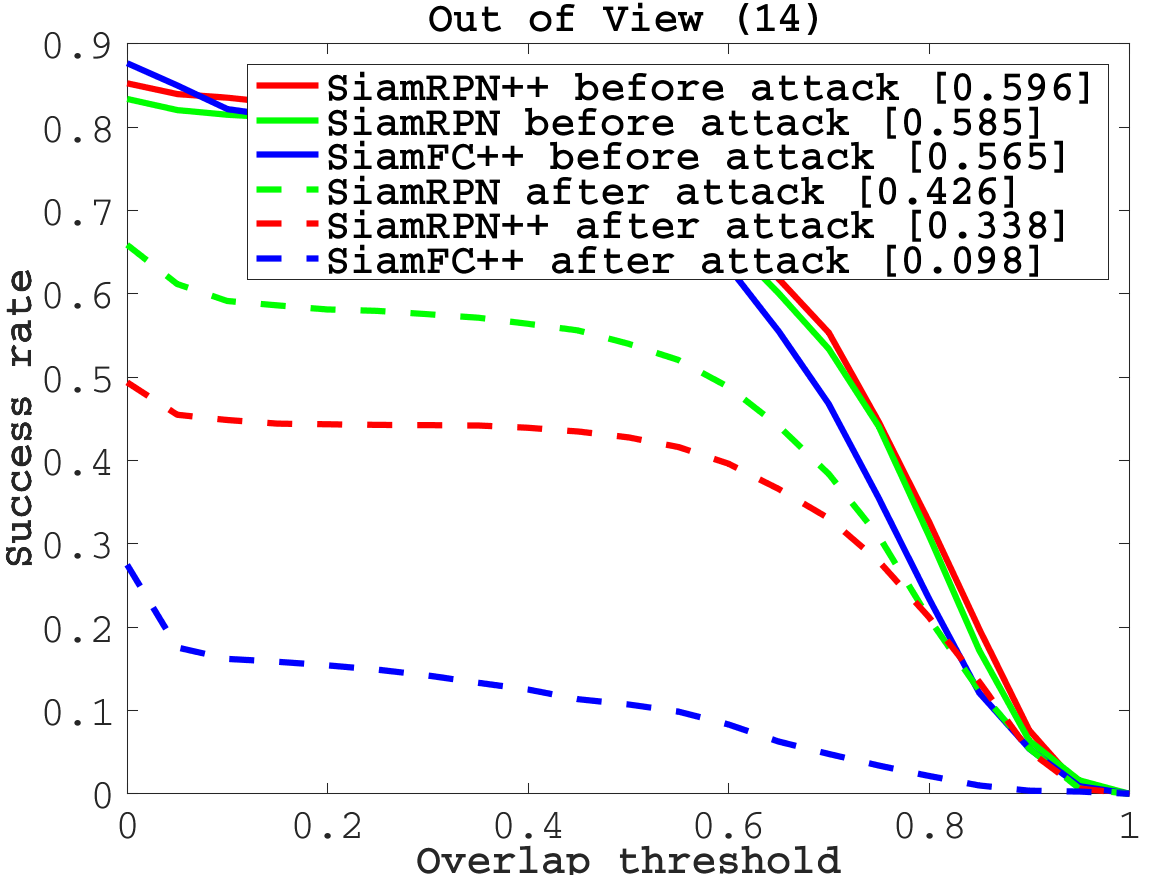
\includegraphics[width=0.32\textwidth]{images_imperceptible/OTB2015/success_plot_OPE_OTB100_OV.png}
%     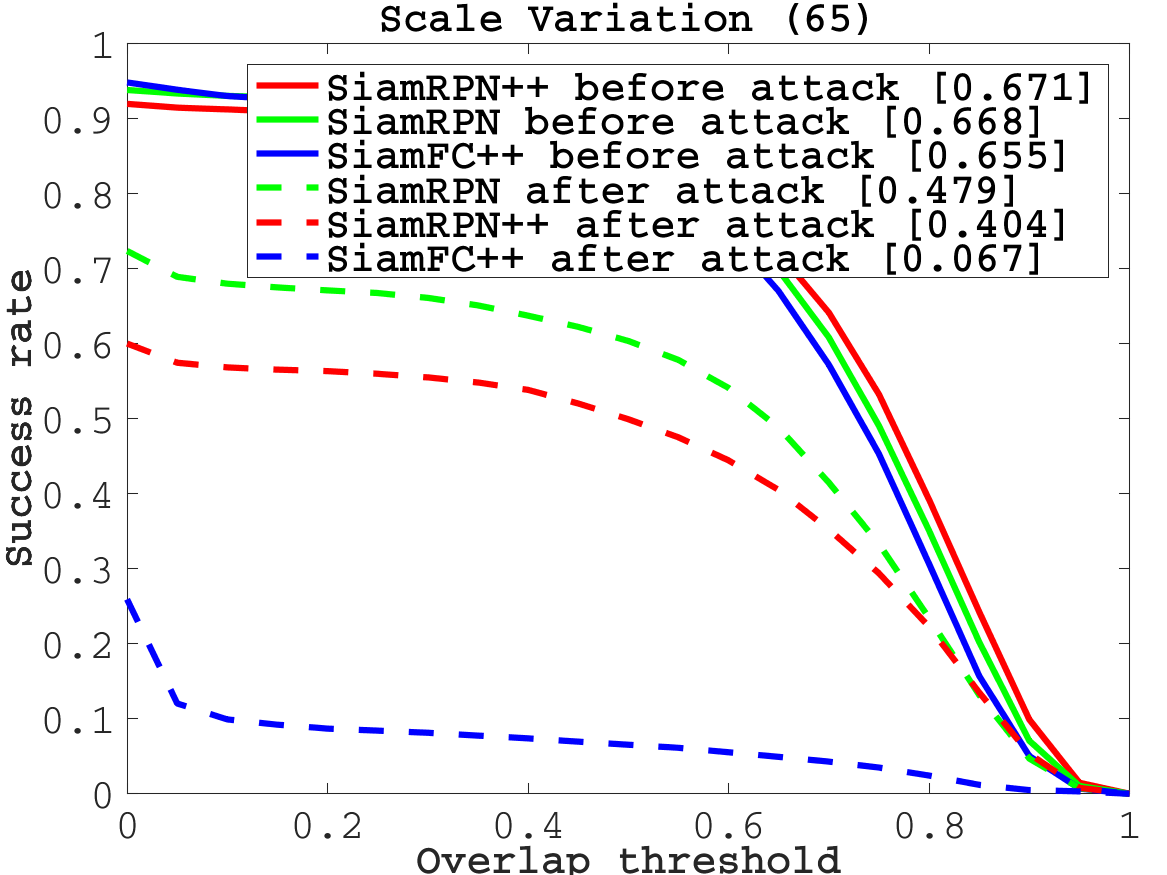
\includegraphics[width=0.32\textwidth]{images_imperceptible/OTB2015/success_plot_OPE_OTB100_SV.png}
%   \end{center}
%       \caption{Untargeted attack results of the different trackers under the 11 attributes: out-of-view (OV), occlusion (OCC), illumination variation (IV), out-of-plane rotation (OPR), scale variation (SV),deformation (DEF), low resolution (LR), fast motion (FM), background clutters (BC), motion blur (MB), and in-plane rotation (IPR). The results show good transferability of our attacks to different tracking architectures, even if the generated perturbations are applied to anchor-based trackers.}
%   \label{fig:attr}
% \end{figure*}

% \restoregeometry

\textbf{Sorry for the inconvenience of reading Fig. 9 caused by the small font size.
We are willing to adjust Fig. 9 font size to make it easier to read on the computer, but because we have added many ablation experiments to revised manuscript, the total number of pages exceeds the maximum page limit for TCSVT (i.e., 14 pages). Therefore we have to remove the analysis of the attack performance for each attribute of the OTB as well as Fig. 9.
}

%%%% 问题 1.4 %%%%
\textit{Also, some recent papers are valued to be referred (2020-2021), to enhance the quality.}

\textbf{Thanks for the good comments. We have added several 2020-2021 related papers to enhance the quality of the revised manuscript. For your convenience of cross review, the new text is given as follows.}

\uline{Some recent research topics which are mostly related to adversarial attack also include digital watermarking [33], 3D face presentation attacks to the face recognition networks [34] and adversarial defense for image classifiers [26].
Xiong \textit{et al.} [33] propose to generate the digital watermarking by slightly modifying the pixel values of video frames to protect video content from unauthorized access. Compared with [33], our purpose of modifying pixel values of video frames is attacking the tracker, instead of detecting the illegal distribution of a digital movie.
Jia \textit{et al.} [34] propose to generate 3D face artifacts to attack the face recognition network. Compared with [34], our method directly modifies the input of the network instead of changing the input of cameras using 3D face artifacts.
Wang \textit{et al.} [26] propose the white-box attack/defense methods for image classifiers. Compared with [26], we focus on attacking the object tracking networks instead of the image classification networks.
}

%%%%%%%%%%%%%%%%% 审稿人 2 %%%%%%%%%%%%%%%%%
\newpage
{\centering\section*{Response Letter to Reviewer \#2}}
\noindent Dear Reviewer \#2:

Thank you very much for your thorough review. Your insightful comments are very helpful for us to improve the quality of the paper. According to your comments and suggestions, we have carefully and extensively revised the manuscript. The main revised parts are highlighted by underlines in the underlined version for your convenience. You will find that all your comments and suggestions are considered and followed. We hope that our revised manuscript is now appropriate for publication in IEEE Transactions on Circuits and Systems for Video Technology.
In addition, point-to-point responses to your comments are given below and highlighted using bold font in line with your comments in order to facilitate cross-referencing.\\[10pt]
\indent We are looking forward to your reply.\\[10pt]
\noindent Yours sincerely,\\
\noindent Zhenbang Li, Yaya Shi, Jin Gao, Shaoru Wang, Bing Li, Pengpeng Liang, Weiming Hu
\\
\\
\\
\noindent Dr. Jin Gao (Contact author)\\
\noindent National Laboratory of Pattern Recognition (NLPR)\\
\noindent Institute of Automation, Chinese Academy of Sciences (CASIA)\\
\noindent Address: No. 95, Zhongguancun East Road, Haidian District,\\
\noindent Beijing 100190, P. R. China\\
\noindent Email: jin.gao@nlpr.ia.ac.cn

\newpage
\textit{In this paper, the authors train a universal adversarial patch to add on both template and search regions of a Siamese based tracker to deteriorate its original performance. The proposed perturbations are video-agnostic, leading to a low computational cost during attack. The experiment validations show that the proposed method achieves favorable attack results on OTB2015, GOT-10k, LaSOT, UAV123, VOT2016, VOT2018 and VOT2019. In addition, the generated perturbations transfer well on other Siamese trackers as well. The idea of this paper is interesting and the experiments are thorough.}

\textbf{Many thanks for your positive comments on the strength of our paper and the novelty of the proposed attack method.}

%%%% 问题 2.1 %%%%
\textit{However, there are some concerns over the implementation, performance and writing. 1. The authors state that training with Ep. 4 leads to an obvious patch on the images while using Eq.5 into the training process results in a less obvious patch. The reviewer considers that giving a constraint (e.g. $l_{\infty}$) on the $p_x$ in Eq.4 can make the perturbation imperceptible intuitively. Please give more analysis on this setting.
Besides, the reviewer hopes to know the reason why give an extra perturbation on the template region. The perturbations on template and search regions look similar, while the authors say that they are different. Please state the difference between the patch application operator on search examples and the operator on template examples.
In addition, the denotations of $A_{\text{paste}}$ in Eq.4 and $A_{\text{add}}$ in Eq.5 seem like the same one.
}

\textbf{
Thanks for the good comment.
Before analyzing whether giving constraint (e.g. $L_{\infty}$) on the $p_x$ in Eq.4 is really lead to imperceptible or not, let us first clarify the concept of the $A_{\text{paste}}$ and $A_{\text{add}}$, which was not explained well in the previous manuscript.}

\textbf{
$A_{\text{paste}}$ means that, in the region where the perturbation is pasted, the pixel values of the original image are \textit{replaced} with the pixel values of the perturbation.
Thus, even if we add constraints to the patch so that the perturbation values are small, when the patch is pasted to the image, it will look like an almost black region, which is obvious rather than imperceptible.}
\textbf{The operator $A_\text{add}$ refers to the injection of our translucent adversarial patch into the search image, \ie, the values of our translucent adversarial patch are \textit{added} to the pixel values of the original image in the $b^{fake}_{\textbf{x}}$ area.
}

\textbf{Next, let us explain the difference between the patch $p$ added to the search image and the perturbation $\delta$ added to the template image. $p$ has a smaller size of $64\times 64$, and added to a larger ($303\times 303$) search image as a fake target.
$\delta$ is the same size ($127\times 127$) as the template image.
% p 通常被加到搜索图像的背景区域,并不会改变真实前景目标区域的像素值。因此如果我们不扰动模板图像的话,总会在真实目标区域有较高的预测。
The adversarial patch is usually added to the background region of the search image and does not change the pixel values in the foreground region where the real target exists. Therefore if we do not add additional perturbation to the template image, the response values of the region where the real target exists on the heatmaps are always high. Thus it is necessary to perturb the template image to cooling down hot regions where the real target exists on the heatmaps and increasing the responses at the position of the \textit{fake target}.
}
\textbf{For your convenience of cross checking, the new added text is shown as follows:}

\uline{
$A_{\text{paste}}$ means that, in the region where the perturbation is pasted, the pixel values of the original image are \textit{replaced} with the pixel values of the perturbation.
The operator $A_\text{add}$ refers to the injection of our translucent adversarial patch into the search image, \ie, the values of our translucent adversarial patch are \textit{added} to the pixel values of the original image in the $b^{fake}_{\textbf{x}}$ area.}

\uline{
The adversarial patch is usually added to the background region of the search image and does not change the pixel values in the foreground region where the real target exists. Therefore if we do not add additional perturbation to the template image, the response values of the region where the real target exists on the heatmaps are always high. Thus it is necessary to perturb the template image to cooling down hot regions where the real target exists on the heatmaps and increasing the responses at the position of the \textit{fake target}.
}


%%%% 问题 2.2 %%%%
\textit{2. I agree with reviewer 3, the ground truth boxes are inaccessible to trackers during the inference. It seems that the authors use the ground truth boxes to generate the fake trajectory in lines 51-57 on page 7. Please clarify it.}

\textbf{
Thanks for the good comment. As suggested, we consider an alternative way to generate the \textit{fake trajectory} without the use of the ground truth boxes.
Specifically, the attacker forces the tracker to follow a fixed direction in each video. For different videos, we assign a random direction from 4 different directions for each of them, each of which consists of shifting the box away by $(\pm 3, \pm 3)$ pixels for each consecutive frame, corresponding to one of the four directions $45^{\circ}, -45^{\circ}, 135^{\circ}, -135^{\circ}$. The attack performance is evaluated on GOT-Val.
The detailed analysis of new added experiment is added in Section IV.E of the revised manuscript. For your convenience in cross-checking, the new text is given as follows.}

\uline{\textit{An Alternative Way to Generate Fake Trajectory.}  Besides the strategy to generate the \textit{fake trajectory} following the real trajectory in Sec.~IV.A, we also consider an alternative way to generate the \textit{fake trajectory}.
Specifically, the attacker forces the tracker to follow a fixed direction in each video. For different videos, we assign a random direction from 4 different directions for each of them, each of which consists of shifting the box away by $(\pm 3, \pm 3)$ pixels for each consecutive frame, corresponding to one of the four directions $45^{\circ}, -45^{\circ}, 135^{\circ}, -135^{\circ}$. The attack performance is evaluated on GOT-Val. As shown in Table \ref{table:direction}, our attack method achieves effective attacks under both of the two different fake trajectory generation ways.}

\begin{table}[t]
  \renewcommand\thetable{XI}
  \centering
  \caption{Influence of two different ways to generate the fake trajectory: following a fixed direction in each video and following the real trajectory. It is evaluated on GOT-Val.}
  \begin{tabular}{@{}rcccc@{}}
  \toprule
  \multirow{2}{*}[-2pt]{Type of the Fake Trajectory} & \multicolumn{2}{c}{Untargeted Attack} & \multicolumn{2}{c}{Targeted Attack} \\ \cmidrule{2-5}
                              & AO                & SR                & AO               & SR               \\ \midrule
  Fixed direction             & 0.175             & 0.144             & 0.845            & 0.897            \\
  Follow the real trajectory      & 0.153             & 0.123             & 0.840            & 0.890            \\ \bottomrule        
  \end{tabular}
  \label{table:direction}
\end{table}

%%%% 问题 2.3 %%%%
\textit{3. For the experiments, the authors should conduct the ablation study on only adding perturbations on the template images or the search regions to show the impact of $p$ and $\delta$.}

\textbf{Thanks for your advice and we have conducted the ablation study on only adding perturbations on the template images or the search regions to show the impact of $p$ and $\delta$.
The detailed analysis of new added experiment is added in Section IV.E of the revised manuscript. For your convenience in cross-checking, the new text is given as follows.}

\uline{\textit{Only Perturb the Template or Search Image.} To analyze the impact of $p$ and $\delta$ in our perturbations, we evaluate the attack performance when only adding perturbations on the template images or the search regions on GOT-Val. The result is shown in Table \ref{table:one_branch}.
For the untargeted attack, only perturbing the template/search image leads to the AO of 0.510/0.714, while perturbing both the template and search image leads to the AO of 0.153.
For the targeted attack, only perturbing the template/search image leads to the AO of 0.156/0.160, while perturbing both the template and search image leads to the AO of 0.840. Experimental results show that perturbing both of them can achieve better attack performance than only perturbing the template/search image.}

\begin{table}[t]
  \renewcommand\thetable{VIII}
  \centering
  \caption{Attack performance comparison when only adding the perturbation on the search/template image. It is evaluated on GOT-Val.}
  \label{table:one_branch}
  \begin{tabular}{@{}cccccc@{}}
  \toprule
  \multirow{2}{*}[-2pt]{Template} & \multirow{2}{*}[-2pt]{Search} & \multicolumn{2}{c}{Untargeted Attack} & \multicolumn{2}{c}{Targeted Attack} \\ \cmidrule{3-6}
                                  &                               & AO                & SR                & AO               & SR               \\ \midrule
  \checkmark                      &                               & 0.510             & 0.567             & 0.156            & 0.106            \\
                                  & \checkmark                    & 0.714             & 0.841             & 0.160            & 0.132            \\
  \checkmark                      & \checkmark                    & 0.153             & 0.123             & 0.840            & 0.890            \\
  \bottomrule
  \end{tabular}
\end{table}

%%%% 问题 2.4 %%%%
\textit{4. As reviewer 1 and reviewer 2 say, the perturbations added to template regions and research regions are not imperceptible, which may be helpful to misguide the tracker. The reviewer considers that adding a similar random pattern on the template and search regions to further illustrate the effectiveness of the proposed method.}

\textbf{To further illustrate the effectiveness of our proposed method, we manually generate similar random patterns and add them on the template and search regions (see Fig. \ref{fig:random}) to show their attack performance. 
Specifically, we design two kinds of random patterns: (1) the random pattern similar to our trained perturbations, and (2) the random pattern generated using zero-mean Gaussian noise with standard deviation 50.0.
We replace the trained perturbations with the above random patterns to attack SiamFC++\_GoogleNet, and experimentally evaluate them on GOT-Val.
As shown in Table \ref{table:noise}, these random patterns cannot effectively attack the tracker.
For your convenience in cross-checking, the new text is given as follows.
}

\begin{table}[t]
  \renewcommand\thetable{VII}
  \centering
  \caption{Attack performance comparison using other random patterns. It is evaluated on GOT-Val.}
  \label{table:noise}
  \begin{tabular}{@{}rcccc@{}}
  \toprule
  \multirow{2}{*}[-1pt]{\begin{tabular}[c]{@{}c@{}}Perturbations used to \\ perfrom attack \end{tabular}} & \multicolumn{2}{c}{Untargeted Attack} & \multicolumn{2}{c}{Targeted Attack}\\ \cmidrule{2-5}
                                                         & AO                                      & SR                               & AO                & SR                  \\ \midrule
  Trained Perturbations                                  & 0.153                                   & 0.123                            & 0.840             & 0.890               \\
  Similar Pattern                                         & 0.736                                   & 0.871                            & 0.153             & 0.118               \\
  Gaussian Noise                                         & 0.740                                   & 0.875                            & 0.144             & 0.101               \\ \bottomrule        
  \end{tabular}
\end{table}
\begin{figure}[t]
  \renewcommand\thefigure{9}
  \centering
  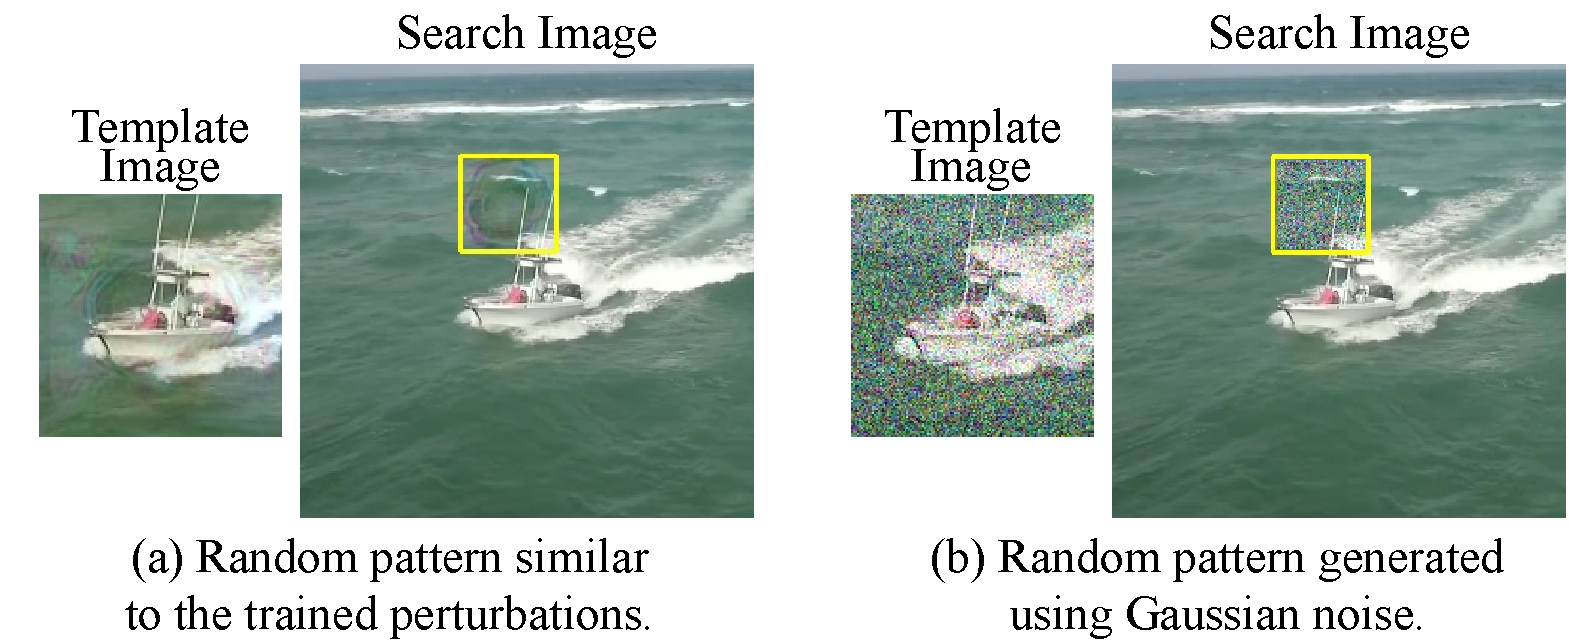
\includegraphics[width=0.8\textwidth]{images_imperceptible/random_gaussian.pdf}
  \caption{Visualization of the manually generated similar random patterns.}
  \label{fig:random}
\end{figure}
\uline{\textit{Use Other Similar Random Patterns.} To further illustrate the effectiveness of our proposed method, we manually generate similar random patterns and add them on the template and search regions (see Fig. \ref{fig:random}) to show their attack performance. 
Specifically, we design two kinds of random patterns: (1) the random pattern similar to our trained perturbations, and (2) the random pattern generated using zero-mean Gaussian noise with standard deviation 50.0.
We replace the trained perturbations with the above random patterns to attack SiamFC++\_GoogleNet, and experimentally evaluate them on GOT-Val.
As shown in Table \ref{table:noise}, these random patterns cannot effectively attack the tracker.
}

%%%% 问题 2.5 %%%%
\textit{
5. There are some minor problems, grammar errors and typos in this paper. The reviewer hopes the authors polish this paper again.}

\textit{- On page 2, ‘1016’ $\rightarrow$ ‘2016’ in line 56. There is a same one in line 47 on page 6.}

\textit{- The denotation of $B_x^{fake}$ in Eq.4 is not clear enough, even though it can be inferred by the later part.}

\textit{- On page 4, ‘imperceptible’ $\rightarrow$ ‘imperceptibly’ in line 57.}

\textit{- The reinitialization of VOT-toolkit should be mentioned in the part of ‘experimental setup’.}

\textit{- On page 7, ‘.(see Table I)’ is a typo.}

\textbf{Thanks for the good comment. We have carefully checked through the whole text and corrected the grammar mistakes and typos. Specifically,}
\textbf{We have replaced ``Experiment results on OTB2015 [11], GOT-10k [12], LaSOT [12], UAV123 [13], VOT1016 [14], VOT2018 [15] and VOT2019 [16]. benchmarks demonstrate the effectiveness and efficiency of our approach.'' with}
``\uline{Experiment results on OTB2015 [11], GOT-10k [12], LaSOT [13], VOT2016 [14], VOT2018 [15] and VOT2019 [16] benchmarks have demonstrated the effectiveness and efficiency of our approach.}''
\textbf{in Section I of the revised manuscript.}

\textbf{We have added the definition of $b_{\textbf{x}}^{fake}$ of Eq.4 as follows:}
``\uline{$b_{\textbf{x}}^{fake} = \{x_0, y_0, x_1, y_1\}$ denotes the coordinates of the upper-left and lower-right corners of the fake target on the search image.}''
\textbf{in Section III.A of the revised manuscript.}

\textbf{We have replaced ``In SiamFC++, the tracker first transforms the paired reference frame $I_1$ and annotation $b_1^{gt}$ to get an template image $\textbf z_1$, and transforms the search frame $I_i$ to get the search image $\textbf x_i$ centered at the position estimated in the previous frame.'' with}
``\uline{In SiamFC++, the tracker first transforms the paired reference frame $I_1$ and annotation $b_1^{gt}$ to get a template image $\textbf z_1$, and transforms the search frame $I_i$ to get the search image $\textbf x_i$ centered at the position estimated in the previous frame.}''
\textbf{in Section III.A of the revised manuscript.}

\textbf{We have replaced ``However, CNN attacks are usually expected imperceptible but the above method has to paste an obviously noticeable fake target patch to tracking frames, which raises the risk of being suspected.'' with}
``\uline{However, CNN attacks are usually expected to be imperceptible whereas the above method has to paste an obviously noticeable \textit{fake target} patch into tracking frames, which raises the risk of being suspected.}''
\textbf{in Section III.A of the revised manuscript.}

\textbf{We have  replaced ``$A_add$ adds the patch into the search image $\textbf x$ at location $(\frac{x_0+x_1}{2},\frac{y_0+y_1}{2})$.'' with}
``\uline{$A_{add}$ adds the patch into the search image $\textbf x$ at location $(\frac{x_0+x_1}{2},\frac{y_0+y_1}{2})$.}''
\textbf{in Section III.B of the revised manuscript.}

\textbf{We have replaced ``We evaluate our video-agnostic perturbations for targeted attacks on several tracking benchmarks, i.e., OTB2015 [11], GOT-10k [12], LaSOT [13], UAV123 [13], VOT1016 [14], VOT2018 [15] and VOT2019 [16].'' with}
``\uline{We evaluate our video-agnostic perturbation method for targeted attacks on several tracking benchmarks, i.e., OTB2015 [11], GOT-10k [12], LaSOT [13], VOT2016 [14], VOT2018 [15] and VOT2019 [16].}''
\textbf{in Section IV.A of the revised manuscript.}

\textbf{We have replaced ``We adopt COCO [63], ILSVRC-VID [64] and the training splits of GOT-10k [12] and LaSOT [13] as our training set. (see Table I)'' with}
``\uline{We adopt COCO [63], ILSVRC-VID [64] and the training splits of GOT-10k [12] and LaSOT [13] as our training set.}''
\textbf{in Section IV.B of the revised manuscript.}

\textbf{We have mentioned the reinitialization of of VOT-toolkit in Section IV.A of the revised manuscript:}
\uline{Different from other datasets, the VOT dataset has a reinitialization module. When the tracker loses the target (\ie, the overlap is zero between the predicted result and the annotation), the tracker will be reinitialized for the remaining frames based on the groundtruth annotation.}

%%%%%%%%%%%%%%%%% 审稿人 3 %%%%%%%%%%%%%%%%%
\clearpage
\newpage
{\centering\section*{Response Letter to Reviewer \#3}}
\noindent Dear Reviewer \#3:

Thank you very much for your thorough review. Your insightful comments are very helpful for us to improve the quality of the paper. According to your comments and suggestions, we have carefully and extensively revised the manuscript. The main revised parts are highlighted by underlines in the underlined version for your convenience. You will find that all your comments and suggestions are considered and followed. We hope that our revised manuscript is now appropriate for publication in IEEE Transactions on Circuits and Systems for Video Technology.
In addition, point-to-point responses to your comments are given below and highlighted using bold font in line with your comments in order to facilitate cross-referencing.\\[10pt]
\indent We are looking forward to your reply.\\[10pt]
\noindent Yours sincerely,\\
\noindent Zhenbang Li, Yaya Shi, Jin Gao, Shaoru Wang, Bing Li, Pengpeng Liang, Weiming Hu
\\
\\
\\
\noindent Dr. Jin Gao (Contact author)\\
\noindent National Laboratory of Pattern Recognition (NLPR)\\
\noindent Institute of Automation, Chinese Academy of Sciences (CASIA)\\
\noindent Address: No. 95, Zhongguancun East Road, Haidian District,\\
\noindent Beijing 100190, P. R. China\\
\noindent Email: jin.gao@nlpr.ia.ac.cn

\newpage

%%%% 问题 3.1 %%%%
\textit{This paper employs the universal perturbation attacks on Siamese visual trackers. There are still the following concerns about the proposed method. 1. As stated in the paper, the proposed method ``does not require gradient optimization or network inference". However, this is a double-edged sword since it resulted in suspicious attacks. Prior works commonly train a network to prevent not only suspicious attacks but also modifying every pixel. I think it's a major problem with this work. I suggest considering a proper strategy to remove/reduce it.}

\textbf{
Thanks for your advice.
Since we can only achieve a balance between the attack efficiency and the perturbation perceptibility, our universal perturbation method may be a double-edged sword as it may result in suspicious attacks. Prior works commonly train a network to prevent not only suspicious attacks but also modifying every pixel. So we also examine a new strategy to perturb the search image so as to reduce the possible suspicion. Specifically, we first convert the search image into YCbCr color space, and then add a perturbation to the entire search image in the Y channel and a different perturbation to a very small region of $64 \times 64$ in the CbCr channel. Different from RGB color space, YCbCr color space encodes a color image similar to human eyes’ retina, which separates the RGB components into a luminance component (Y) and two chrominance components (Cb as blue projection and Cr as red projection). We choose YCbCr color space since its color channels are less correlated than RGB [65]. Moreover, the CbCr channels are less sensitive to the human vision system than the Y channel [65], which means that the patch added in the CbCr channels has better performance of transparency.
The detailed analysis of new added experiment is added in Section IV.D of the revised manuscript.
For your convenience in cross-checking, the new text is given as follows.}

\begin{figure}[t]
  \renewcommand\thefigure{8}
  \centering
  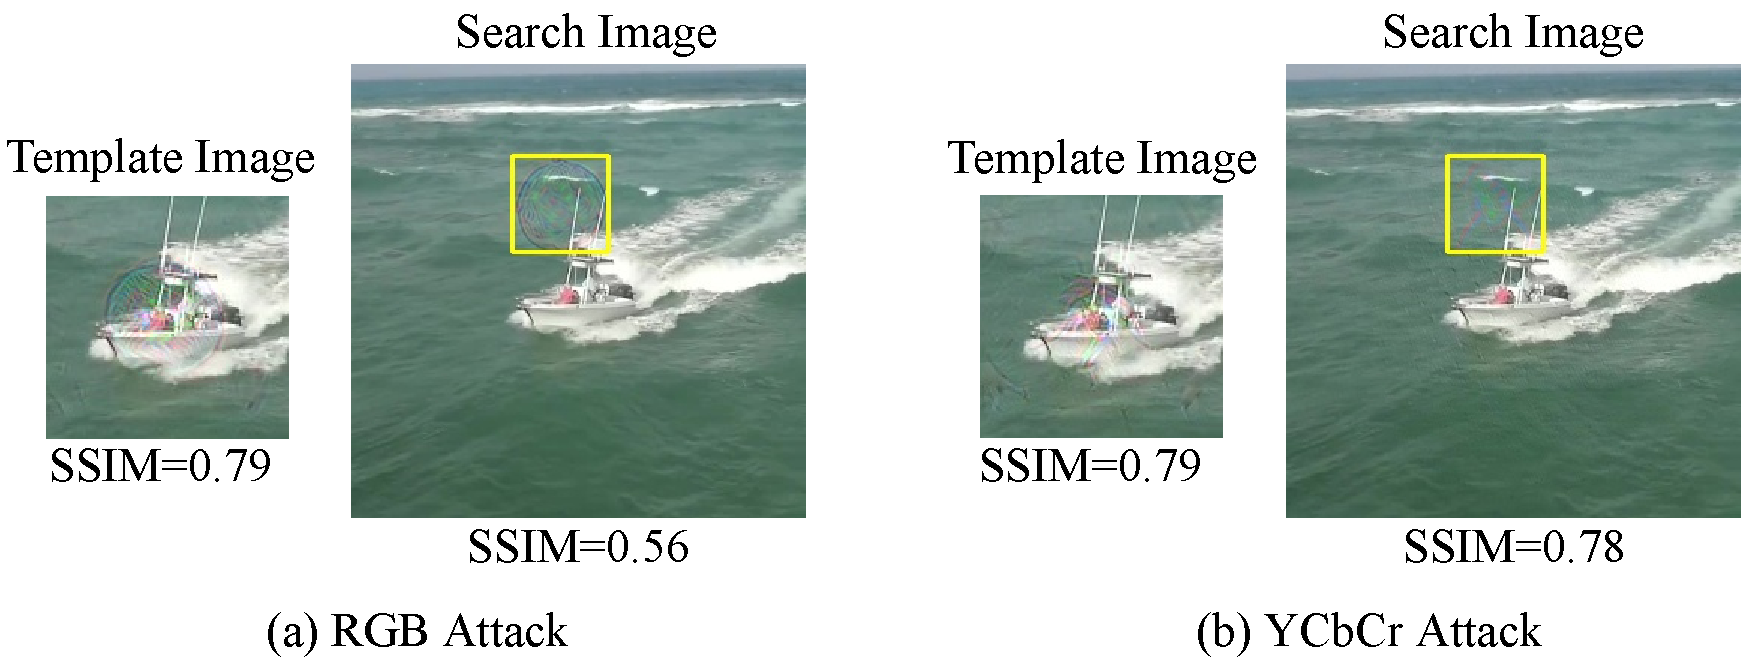
\includegraphics[width=.8\textwidth]{images_imperceptible/1.pdf}
  \caption{Visualization of the perturbations in attacking the different RGB and YCbCr color spaces. Note that the perturbation of the search image in the Y channel results in SSIM value of 0.95 outside the added patch area, which slightly deteriorate the imperceptibility.}
  \label{fig:YCbCr}
\end{figure}

\begin{table}[t]
  \renewcommand\thetable{VI}
  \centering
  \caption{Comparison between attacking the different RGB and YCbCr color spaces. Attacking the YCbCr color space means we first convert the search image into YCbCr color space, and then add a perturbation to the entire search image in the Y channel and a different perturbation to a very small region of $64 \times 64$ in the CbCr channel. The attack performance is evaluated on GOT-Val.}
  \label{table:perturb}
  \begin{tabular}{@{}rcccccc@{}}
  \toprule
  \multirow{2}{*}[-1pt]{\begin{tabular}[c]{@{}c@{}}Different Color\\ Space Attack\end{tabular}} & \multicolumn{2}{c}{Untargeted Attack} & \multicolumn{2}{c}{Targeted Attack} & \multicolumn{2}{c}{SSIM} \\ \cmidrule{2-7}
                                                         & AO                                      & SR                               & AO                & SR                   & $\delta$          & $p$  \\ \midrule
  RGB Attack                                             & 0.153                                   & 0.123                            & 0.840             & 0.890                & 0.56              & 0.79 \\
  YCbCr Attack                                           & 0.246                                   & 0.227                            & 0.682             & 0.756                & 0.78              & 0.79 \\ \bottomrule        
  \end{tabular}
\end{table}

\uline{\textit{Analyses of the Perceptibility of Our Perturbations}
Since we can only achieve a balance between the attack efficiency and the perturbation perceptibility, our universal perturbation method may be a double-edged sword as it may result in suspicious attacks. Prior works commonly train a network to prevent not only suspicious attacks but also modifying every pixel. So we also examine a new strategy to perturb the search image so as to reduce the possible suspicion. Specifically, we first convert the search image into YCbCr color space, and then add a perturbation to the entire search image in the Y channel and a different perturbation to a very small region of $64 \times 64$ in the CbCr channel. Different from RGB color space, YCbCr color space encodes a color image similar to human eyes’ retina, which separates the RGB components into a luminance component (Y) and two chrominance components (Cb as blue projection and Cr as red projection). We choose YCbCr color space since its color channels are less correlated than RGB [65]. Moreover, the CbCr channels are less sensitive to the human vision system than the Y channel [65], which means that the patch added in the CbCr channels has better performance of transparency.
For the template image, we also convert it into YCbCr color space, and then add the perturbation to the entire template image in all YCbCr channels. The perturbed template and search images are finally converted into RGB color space and fed into the tracking network. The other steps of the training process are the same to the attack method in Sec.~III. As shown in Table \ref{table:perturb}, the performance of attacking the YCbCr color space is slightly degraded compared to the RGB color space. However, attacking the YCbCr color space brings better imperceptibility (see Fig. \ref{fig:YCbCr}). Compared with the RGB space, the SSIM value for the search image increases from 0.56 to 0.78. Note that the perturbation of the search image in the Y channel results in SSIM value of 0.95 outside the added patch area, which slightly deteriorate the imperceptibility.
}

%%%% 问题 3.2 %%%%
\textit{2. The proposed method and offline training phase should be explained more clearly. For instance, the termination of offline training or offline optimization is missed affecting perturbation values.}

\textbf{Thanks for the good comment. As suggested, we have explained in detail the perturbation update process in offline training.
The detailed analysis is added in Section III.B of the revised manuscript.
For your convenience in cross-checking, the new text is given as follows.}

\uline{Before introducing our perturbation update process in offline training, we first revisit the popular adversarial example generation methods (\eg,~[55], [56]). One of the simplest methods to generate adversarial image $I^{adv}$ is FGSM~[55] and works by linearizing the loss function around the network weights and obtaining an optimal max-norm constrained perturbation for generating the adversarial image:}
\begin{equation}
    \renewcommand\theequation{11}
    I^{adv} = I + \epsilon \cdot \text{ sign} \bigl( \nabla_I J(I, y_{true})  \bigr),
    \vspace{-0.1cm}
\end{equation}
\uline{where $I$ is the input clean image, and the values of its pixels are integer numbers in the range [0, 255]. $y_{true}$ is the true label for the image $I$, $J(I, y_{true})$ is the cost function for training the neural network, and $\epsilon$ is a hyper-parameter to be chosen. A straightforward way to extend the above method is applying it multiple times with small step size. This leads to Basic Iterative Method (BIM) introduced in [56]:}
\begin{equation}
  \renewcommand\theequation{12}
    \begin{gathered}
        I_0^{adv} = I, \\
        I_{N+1}^{adv} = Clip_{I, \epsilon}\left\{I_N^{adv}+\epsilon \cdot \text{ sign}(\nabla_I J(I_N^{adv},y_{true}))\right\},
    \end{gathered}
\end{equation}
\uline{where the pixel values of intermediate results are clipped after each step to ensure that they are in
an $\epsilon$-neighbourhood of the original image. The BIM method can be easily made into an attacker for a specific desired target class, called Iterative Target Class Method [56]:}
\begin{equation}
  \renewcommand\theequation{13}
  \begin{gathered}
      I_0^{adv} = I,\\
      I_{N+1}^{adv} = Clip_{I, \epsilon}\left\{I_N^{adv}-\epsilon \cdot \text{ sign}(\nabla_I J(I_N^{adv},y_{target}))\right\}.
  \end{gathered}
\end{equation}

\uline{We utilize this Iterative Target Class Method to update our perturbation values during the training process. To achieve a balance between the attack efficiency and the perturbation perceptibility, we constrain the perturbation values in the loss function of Eq.~(10) instead of using the clip operation. At each training step, our perturbations are updated as follows:}
\begin{equation}
\renewcommand\theequation{14}
\delta_{k+1} = \delta_{k} - \epsilon_1 \cdot \text{sign}(\nabla_{\delta_k}L)
\end{equation}
\begin{equation}
\renewcommand\theequation{15}
p_{k+1} = p_{k} - \epsilon_2 \cdot \text{sign}(\nabla_{p_k}L),
\end{equation}

\textit{3. The descriptions of figures and tables are not self-explanatory.}

\textbf{Thanks for your advice and we have rewritten the descriptions of figures and tables. The modification is shown as follows for the convience of cross checking.}

\textbf{In Table IV, we have replaced ``Compared with baselines on perturbed GOT-Val dataset.'' with}
\uline{``Comparison of attack performance with 2 baseline methods on GOT-Val in terms of AO. Baseline-1 performs untargeted attacks based on the UAP [9] method. Baseline-2 performs targeted attacks based on the adversarial patch [50] method.''}
\textbf{in Section IV.D of the revised manuscript.}

\textbf{In Table IX, we have replaced ``Contribution of each loss on GOT-Val.'' with}
\uline{``Analysis of the impact of each loss component on GOT-Val.''}
\textbf{in Section IV.E of the revised manuscript.}

\textbf{In Table XII, we have replaced ``Transferability to different backbones on GOT-Val.'' with}
\uline{``Transferability to different backbones of our perturbations trained on SiamFC++\_GoogleNet. It is evaluated on GOT-Val.''}
\textbf{in Section IV.F of the revised manuscript.}

\textbf{In Table XIII, we have replaced ``Transferability to different tracking architectures on OTB2015.'' with}
\uline{``Transferability to different tracking architectures of our perturbations trained on SiamFC++\_GoogleNet. It is evaluated on OTB2015.''}
\textbf{in Section IV.F of the revised manuscript.}

% table 14
\textbf{In Table XIV, we have replaced ``Untargeted attack: Precision score on OTB2015.'' with}
\uline{``State-of-the-art comparison of untargeted attack performance on OTB2015 in terms of precision score.''}
\textbf{in Section IV.G of the revised manuscript.}

% table 15
\textbf{In Table XV, we have replaced ``Targeted attack: Precision score on OTB2015.'' with}
\uline{``State-of-the-art comparison of targeted attack performance on OTB2015 in terms of precision score.''}
\textbf{in Section IV.G of the revised manuscript.}

% figure 4
\textbf{In Figure 4, we have replaced ``Results of targeted attacks where the tracker is forced to follow a predefined \textit{fake trajectory} (indicated by the yellow targeted bounding box).'' with}
\uline{``Results of targeted attacks where the tracker is forced to follow a predefined \textit{fake trajectory} $B^{fake}=\{b^{fake}_i\}_1^{T}$ (indicated by the yellow bounding boxes). The \textit{fake trajectory} follows the real trajectory $B^{gt}=\{b^{gt}_i\}_1^T$ (indicated by the red bounding boxes) except that the adjacent boundaries of $b^{fake}_i$ and $b^{gt}_i$ are 2 pixels apart.''}


\textit{4. I suggest adding the advantages \& limitations of the proposed method after experimental analysis and future works to the conclusion.}

\textbf{Thanks for the good commenet. As suggested, we have added the advantages \& limitations of the proposed method after experimental analysis and future works to the conclusion. For your convenience in cross-checking, the new text is given as follows.}

\uline{In summary, compared with other attack methods, our method has two key advantages. First, the proposed attack method only needs to perform the addition operations to deploy the adversarial information for any novel video without gradient optimization or network inference, making it possible to attack a real-world online-tracking system when we can not get access to the limited computational resources. Second, the proposed perturbations show good transferability to other anchor-free or anchor-based trackers. The main limitation of our work is that the translucent perturbations my result in suspicious attacks.
In the future work, we expect that it will be possible to further reduce the possible suspicion by increasing the perturbation's imperceptibility while maintaining the attack efficiency.}

\textit{5. Some of the experiments require more explanations. For example, transferability has been investigated by different backbones \& architectures. It's needed to mention these experiments are with/without the training phase or not.}

\textbf{Thanks for the good comment. These experiments do not need the training phase and we have clarified this in Section IV.F of the revised manuscript. For your convenience in cross-checking, the new text is given as follows.}

\uline{In this part, we analyze the transferability of our proposed attack method. Specifically, we directly apply our perturbations trained on SiamFC++\_GoogleNet to other tracking networks including SiamFC++\_ShuffleNet, SiamFC++\_AlexNet, SiamPRN, SiamRPN++ and Ocean.}

\textit{6. In experiments, I suggest considering two scenarios of different directions and trajectories.}

\textbf{Thanks for the good comment. As suggest, we consider an alternative way to generate the \textit{fake trajectory} without the use of the ground truth boxes.
Specifically, the attacker forces the tracker to follow a fixed direction in each video. For different videos, we assign a random direction from 4 different directions for each of them, each of which consists of shifting the box away by $(\pm 3, \pm 3)$ pixels for each consecutive frame, corresponding to one of the four directions $45^{\circ}, -45^{\circ}, 135^{\circ}, -135^{\circ}$. The attack performance is evaluated on GOT-Val.
The detailed analysis of new added experiment is added in Section IV.E of the revised manuscript. For your convenience in cross-checking, the new text is given as follows.}

\uline{\textit{An Alternative Way to Generate Fake Trajectory.}  Besides the strategy to generate the \textit{fake trajectory} following the real trajectory in Sec.~IV.A, we also consider an alternative way to generate the \textit{fake trajectory}.
Specifically, the attacker forces the tracker to follow a fixed direction in each video. For different videos, we assign a random direction from 4 different directions for each of them, each of which consists of shifting the box away by $(\pm 3, \pm 3)$ pixels for each consecutive frame, corresponding to one of the four directions $45^{\circ}, -45^{\circ}, 135^{\circ}, -135^{\circ}$. The attack performance is evaluated on GOT-Val. As shown in Table \ref{table:direction}, our attack method achieves effective attacks under both of the two different fake trajectory generation ways.}

\begin{table}[t]
  \renewcommand\thetable{\ref{table:direction}}
  \centering
  \caption{Influence of two different ways to generate the fake trajectory: following a fixed direction in each video and following the real trajectory. It is evaluated on GOT-Val.}
  \begin{tabular}{@{}rcccc@{}}
  \toprule
  \multirow{2}{*}[-2pt]{Type of the Fake Trajectory} & \multicolumn{2}{c}{Untargeted Attack} & \multicolumn{2}{c}{Targeted Attack} \\ \cmidrule{2-5}
                              & AO                & SR                & AO               & SR               \\ \midrule
  Fixed direction             & 0.175             & 0.144             & 0.845            & 0.897            \\
  Follow the real trajectory  & 0.153             & 0.123             & 0.840            & 0.890            \\ \bottomrule        
  \end{tabular}
\end{table}

\textit{7. There are still some typo and grammar mistakes in the paper.}

\textbf{Thanks for the good comment. We have carefully checked through the whole text and corrected the grammar mistakes and typos. Specifically,}
\textbf{We have replaced ``Experiment results on OTB2015 [11], GOT-10k [12], LaSOT [12], UAV123 [13], VOT1016 [14], VOT2018 [15] and VOT2019 [16]. benchmarks demonstrate the effectiveness and efficiency of our approach.'' with}
``\uline{Experiment results on OTB2015 [11], GOT-10k [12], LaSOT [13], VOT2016 [14], VOT2018 [15] and VOT2019 [16] benchmarks have demonstrated the effectiveness and efficiency of our approach.}''
\textbf{in Section I of the revised manuscript.}

\textbf{We have replaced ``In SiamFC++, the tracker first transforms the paired reference frame $I_1$ and annotation $b_1^{gt}$ to get an template image $\textbf z_1$, and transforms the search frame $I_i$ to get the search image $\textbf x_i$ centered at the position estimated in the previous frame.'' with}
``\uline{In SiamFC++, the tracker first transforms the paired reference frame $I_1$ and annotation $b_1^{gt}$ to get a template image $\textbf z_1$, and transforms the search frame $I_i$ to get the search image $\textbf x_i$ centered at the position estimated in the previous frame.}''
\textbf{in Section III.A of the revised manuscript.}

\textbf{We have replaced ``However, CNN attacks are usually expected imperceptible but the above method has to paste an obviously noticeable fake target patch to tracking frames, which raises the risk of being suspected.'' with}
``\uline{However, CNN attacks are usually expected to be imperceptible whereas the above method has to paste an obviously noticeable \textit{fake target} patch into tracking frames, which raises the risk of being suspected.}''
\textbf{in Section III.A of the revised manuscript.}

\textbf{We have  replaced ``$A_add$ adds the patch into the search image $\textbf x$ at location $(\frac{x_0+x_1}{2},\frac{y_0+y_1}{2})$.'' with}
``\uline{$A_{add}$ adds the patch into the search image $\textbf x$ at location $(\frac{x_0+x_1}{2},\frac{y_0+y_1}{2})$.}''
\textbf{in Section III.B of the revised manuscript.}

\textbf{We have replaced ``We evaluate our video-agnostic perturbations for targeted attacks on several tracking benchmarks, i.e., OTB2015 [11], GOT-10k [12], LaSOT [13], UAV123 [13], VOT1016 [14], VOT2018 [15] and VOT2019 [16].'' with}
``\uline{We evaluate our video-agnostic perturbation method for targeted attacks on several tracking benchmarks, i.e., OTB2015 [11], GOT-10k [12], LaSOT [13], VOT2016 [14], VOT2018 [15] and VOT2019 [16].}''
\textbf{in Section IV.A of the revised manuscript.}

\textbf{We have replaced ``We adopt COCO [63], ILSVRC-VID [64] and the training splits of GOT-10k [12] and LaSOT [13] as our training set. (see Table I)'' with}
``\uline{We adopt COCO [63], ILSVRC-VID [64] and the training splits of GOT-10k [12] and LaSOT [13] as our training set.}''
\textbf{in Section IV.B of the revised manuscript.}

\textit{8. Missing key ref : "Deep Learning for Visual Tracking: A Comprehensive Survey," in IEEE Transactions on Intelligent Transportation Systems, 2021.}

\textbf{Thanks for the good comment. We have cited this paper at Section II of the revised manuscript.  For your convenience in cross-checking, the new text is given as follows.}

\uline{A comprehensive survey of the related trackers is beyond the scope of this paper, please refer to [25] for a thorough survey.}

%%%%%%%%%%%%%%%%% 审稿人 4 %%%%%%%%%%%%%%%%%
\clearpage
\newpage
{\centering\section*{Response Letter to Reviewer \#4}}
\noindent Dear Reviewer \#4:

Thank you very much for your thorough review. Your insightful comments are very helpful for us to improve the quality of the paper. According to your comments and suggestions, we have carefully and extensively revised the manuscript. The main revised parts are highlighted by underlines in the underlined version for your convenience. You will find that all your comments and suggestions are considered and followed. We hope that our revised manuscript is now appropriate for publication in IEEE Transactions on Circuits and Systems for Video Technology.
In addition, point-to-point responses to your comments are given below and highlighted using bold font in line with your comments in order to facilitate cross-referencing.\\[10pt]
\indent We are looking forward to your reply.\\[10pt]
\noindent Yours sincerely,\\
\noindent Zhenbang Li, Yaya Shi, Jin Gao, Shaoru Wang, Bing Li, Pengpeng Liang, Weiming Hu
\\
\\
\\
\noindent Dr. Jin Gao (Contact author)\\
\noindent National Laboratory of Pattern Recognition (NLPR)\\
\noindent Institute of Automation, Chinese Academy of Sciences (CASIA)\\
\noindent Address: No. 95, Zhongguancun East Road, Haidian District,\\
\noindent Beijing 100190, P. R. China\\
\noindent Email: jin.gao@nlpr.ia.ac.cn

\newpage
\textit{This paper proposes a universal targeted attacks method on Siamese visual tracking task. It seems that the method is feasible and somewhat novel.}

\textbf{Many thanks for your positive comments on the strength of our paper and the novelty of the proposed attack method.}

\textit{My major concern is that the writing and organization need to be carefully modified and optimized. Besides, 1. Authors are focused on the anchor-free tracker in the experiments, but the anchor-free Siamese trackers are not well mentioned. I suggest the authors to include the discussion of state-of-the-art of other similar approaches (e.g., FCOT, SiamCAR, OCEAN, et. al.).}

\textbf{We have discussed several state-of-the-art anchor free Siamese trackers at the related work. For your convenience of cross review, the new text is given as follows.}

\uline{In this anchor-free paradigm, many recent works (e.g., [20], [21], [22]) are dedicated to more robust and efficient visual tracking based on various anchor-free settings.
% Ocean
Ocean [20] directly predicts the position and scale of target objects in an anchor-free fashion; since each sample position in groundtruth boxes is well trained, the tracker is capable of rectifying inexact predictions of target objects during inference.
% FCOT
FCOT [21] introduces an online regression model generator (RMG) based on the carefully designed anchor-free box regression branch, which enables the tracker to be more effective in handling target deformation during tracking procedure.
%  SiamCAR
SiamCAR [22] is both anchor and proposal free, and takes one unique response map to predict object location and bounding box directly; this setting significantly reduces the number of hyper-parameters, which keeps the tracker from complicated parameter tuning and makes the tracker significantly simpler, especially in training.
}

\textbf{Besides, we have evaluated the transferability to the anchor free tracker OCEAN in Setcion IV.F of the revised manuscript. For your convenience of cross review, the new text is given as follows.}

\begin{table}[t]
  \renewcommand\thetable{XIII}
  \centering
  \caption{Transferability to different tracking architectures of our perturbations trained on SiamFC++\_GoogleNet. It is evaluated on OTB2015.}
  \begin{tabular}{rcccc} 
  \toprule
  \multirow{2}{*}[-2pt]{Trackers} & \multicolumn{2}{c}{Before Attack} & \multicolumn{2}{c}{Untargeted Attack}  \\
  \cmidrule{2-5}
                            & AO & Precision              & AO    & Precision \\ \midrule
  SiamRPN++ [24]            & 0.676   & 0.879             & 0.418 & 0.556     \\
  SiamRPN [23]              & 0.666   & 0.876             & 0.483 & 0.643     \\
  Ocean [20]                & 0.672   & 0.902             & 0.237 & 0.282     \\ \bottomrule
  \end{tabular}
  \label{tab:arch}
\end{table}
\uline{\textit{Transferability to Different Tracking Architectures.} We also evaluate the transferability of our attacks when applying the perturbations to three more state-of-the-art trackers: SiamRPN [23], SiamRPN++ [24] and Ocean [20]. SiamRPN and SiamRPN++ are anchor-based trackers, and Ocean is an anchor-free tracker. The experimental results are shown in Table \ref{tab:arch}. In the case of SiamRPN, the AO with respect to the real trajectory decreases from 0.666 to 0.483 and the performance of SiamRPN++ is decreased from 0.676 to 0.418. In the case of Ocean, the AO with respect to the real trajectory decreases from 0.902 to 0.282. The results show good transferability of our attacks to different tracking architectures, even if the generated perturbations are applied to anchor-based trackers.
}

\textit{2. The model is trained based on Eq.11 and Eq.12. It is not clear why the sign function is introduced. It is also suggested to describe the derivation of these two equations in detail.}

\textbf{Thanks for the good comment. As suggested, we have explained in detail the perturbation update process in offline training.
The detailed analysis is added in Section III.B of the revised manuscript.
For your convenience in cross-checking, the new text is given as follows.}

\uline{Before introducing our perturbation update process in offline training, we first revisit the popular adversarial example generation methods (\eg,~[55], [56]). One of the simplest methods to generate adversarial image $I^{adv}$ is FGSM~[55] and works by linearizing the loss function around the network weights and obtaining an optimal max-norm constrained perturbation for generating the adversarial image:}
\begin{equation}
    \renewcommand\theequation{11}
    I^{adv} = I + \epsilon \cdot \text{ sign} \bigl( \nabla_I J(I, y_{true})  \bigr),
    \vspace{-0.1cm}
\end{equation}
\uline{where $I$ is the input clean image, and the values of its pixels are integer numbers in the range [0, 255]. $y_{true}$ is the true label for the image $I$, $J(I, y_{true})$ is the cost function for training the neural network, and $\epsilon$ is a hyper-parameter to be chosen. A straightforward way to extend the above method is applying it multiple times with small step size. This leads to Basic Iterative Method (BIM) introduced in [56]:}
\begin{equation}
    \renewcommand\theequation{12}
    \begin{gathered}
        I_0^{adv} = I, \\
        I_{N+1}^{adv} = Clip_{I, \epsilon}\left\{I_N^{adv}+\epsilon \cdot \text{ sign}(\nabla_I J(I_N^{adv},y_{true}))\right\},
    \end{gathered}
\end{equation}
\uline{where the pixel values of intermediate results are clipped after each step to ensure that they are in
an $\epsilon$-neighbourhood of the original image. The BIM method can be easily made into an attacker for a specific desired target class, called Iterative Target Class Method [56]:}
\begin{equation}
  \renewcommand\theequation{13}
  \begin{gathered}
      I_0^{adv} = I,\\
      I_{N+1}^{adv} = Clip_{I, \epsilon}\left\{I_N^{adv}-\epsilon \cdot \text{ sign}(\nabla_I J(I_N^{adv},y_{target}))\right\}.
  \end{gathered}
  \label{equ:itcm}
\end{equation}

\uline{We utilize this Iterative Target Class Method to update our perturbation values during the training process. To achieve a balance between the attack efficiency and the perturbation perceptibility, we constrain the perturbation values in the loss function of Eq.~(10) instead of using the clip operation. At each training step, our perturbations are updated as follows:}
\begin{equation}
  \renewcommand\theequation{14}
  \delta_{k+1} = \delta_{k} - \epsilon_1 \cdot \text{sign}(\nabla_{\delta_k}L)
  \end{equation}
  \begin{equation}
  \renewcommand\theequation{15}
  p_{k+1} = p_{k} - \epsilon_2 \cdot \text{sign}(\nabla_{p_k}L),
\end{equation}


\textit{3. The format of all the Tables is suggested to be unified.}

\textbf{Thanks for the good comment. We have unified the format of all the Tables in the revised manuscript.}

\textit{4. There are many typos in the paper, including but not limited to the following errors:}

\textit{(a) In the third line below Eq.7, $A_{a}dd$ should be $A_{add}$.}

\textit{(b) In page 2, difference datasets GOT-10K[12], LaSOT [12] cite the same reference.}

\textit{(c) In page 3, Subsection A of Section 3, “to get an template image” should be “to get a template image”.}

\textbf{Thanks for the good comment. We have carefully checked through the whole text and corrected the grammar mistakes and typos. Specifically,}
\textbf{We have replaced ``Experiment results on OTB2015 [11], GOT-10k [12], LaSOT [12], UAV123 [13], VOT1016 [14], VOT2018 [15] and VOT2019 [16]. benchmarks demonstrate the effectiveness and efficiency of our approach.'' with}
``\uline{Experiment results on OTB2015 [11], GOT-10k [12], LaSOT [13], VOT2016 [14], VOT2018 [15] and VOT2019 [16] benchmarks have demonstrated the effectiveness and efficiency of our approach.}''
\textbf{in Section I of the revised manuscript.}

\textbf{We have replaced ``In SiamFC++, the tracker first transforms the paired reference frame $I_1$ and annotation $b_1^{gt}$ to get an template image $\textbf z_1$, and transforms the search frame $I_i$ to get the search image $\textbf x_i$ centered at the position estimated in the previous frame.'' with}
``\uline{In SiamFC++, the tracker first transforms the paired reference frame $I_1$ and annotation $b_1^{gt}$ to get a template image $\textbf z_1$, and transforms the search frame $I_i$ to get the search image $\textbf x_i$ centered at the position estimated in the previous frame.}''
\textbf{in Section III.A of the revised manuscript.}

\textbf{We have replaced ``However, CNN attacks are usually expected imperceptible but the above method has to paste an obviously noticeable fake target patch to tracking frames, which raises the risk of being suspected.'' with}
``\uline{However, CNN attacks are usually expected to be imperceptible whereas the above method has to paste an obviously noticeable \textit{fake target} patch into tracking frames, which raises the risk of being suspected.}''
\textbf{in Section III.A of the revised manuscript.}

\textbf{We have  replaced ``$A_add$ adds the patch into the search image $\textbf x$ at location $(\frac{x_0+x_1}{2},\frac{y_0+y_1}{2})$.'' with}
``\uline{$A_{add}$ adds the patch into the search image $\textbf x$ at location $(\frac{x_0+x_1}{2},\frac{y_0+y_1}{2})$.}''
\textbf{in Section III.B of the revised manuscript.}

\textbf{We have replaced ``We evaluate our video-agnostic perturbations for targeted attacks on several tracking benchmarks, i.e., OTB2015 [11], GOT-10k [12], LaSOT [13], UAV123 [13], VOT1016 [14], VOT2018 [15] and VOT2019 [16].'' with}
``\uline{We evaluate our video-agnostic perturbation method for targeted attacks on several tracking benchmarks, i.e., OTB2015 [11], GOT-10k [12], LaSOT [13], VOT2016 [14], VOT2018 [15] and VOT2019 [16].}''
\textbf{in Section IV.A of the revised manuscript.}

\textbf{We have replaced ``We adopt COCO [63], ILSVRC-VID [64] and the training splits of GOT-10k [12] and LaSOT [13] as our training set. (see Table I)'' with}
``\uline{We adopt COCO [63], ILSVRC-VID [64] and the training splits of GOT-10k [12] and LaSOT [13] as our training set.}''
\textbf{in Section IV.B of the revised manuscript.}

%\normalem
% \bibliographystyle{IEEEtran}
% \bibliography{ref.bib}

\end{document}

